% Options for packages loaded elsewhere
\PassOptionsToPackage{unicode}{hyperref}
\PassOptionsToPackage{hyphens}{url}
\PassOptionsToPackage{dvipsnames,svgnames,x11names}{xcolor}
%
\documentclass[
  letterpaper,
  DIV=11,
  numbers=noendperiod]{scrartcl}

\usepackage{amsmath,amssymb}
\usepackage{lmodern}
\usepackage{iftex}
\ifPDFTeX
  \usepackage[T1]{fontenc}
  \usepackage[utf8]{inputenc}
  \usepackage{textcomp} % provide euro and other symbols
\else % if luatex or xetex
  \usepackage{unicode-math}
  \defaultfontfeatures{Scale=MatchLowercase}
  \defaultfontfeatures[\rmfamily]{Ligatures=TeX,Scale=1}
\fi
% Use upquote if available, for straight quotes in verbatim environments
\IfFileExists{upquote.sty}{\usepackage{upquote}}{}
\IfFileExists{microtype.sty}{% use microtype if available
  \usepackage[]{microtype}
  \UseMicrotypeSet[protrusion]{basicmath} % disable protrusion for tt fonts
}{}
\makeatletter
\@ifundefined{KOMAClassName}{% if non-KOMA class
  \IfFileExists{parskip.sty}{%
    \usepackage{parskip}
  }{% else
    \setlength{\parindent}{0pt}
    \setlength{\parskip}{6pt plus 2pt minus 1pt}}
}{% if KOMA class
  \KOMAoptions{parskip=half}}
\makeatother
\usepackage{xcolor}
\setlength{\emergencystretch}{3em} % prevent overfull lines
\setcounter{secnumdepth}{-\maxdimen} % remove section numbering
% Make \paragraph and \subparagraph free-standing
\ifx\paragraph\undefined\else
  \let\oldparagraph\paragraph
  \renewcommand{\paragraph}[1]{\oldparagraph{#1}\mbox{}}
\fi
\ifx\subparagraph\undefined\else
  \let\oldsubparagraph\subparagraph
  \renewcommand{\subparagraph}[1]{\oldsubparagraph{#1}\mbox{}}
\fi

\usepackage{color}
\usepackage{fancyvrb}
\newcommand{\VerbBar}{|}
\newcommand{\VERB}{\Verb[commandchars=\\\{\}]}
\DefineVerbatimEnvironment{Highlighting}{Verbatim}{commandchars=\\\{\}}
% Add ',fontsize=\small' for more characters per line
\usepackage{framed}
\definecolor{shadecolor}{RGB}{241,243,245}
\newenvironment{Shaded}{\begin{snugshade}}{\end{snugshade}}
\newcommand{\AlertTok}[1]{\textcolor[rgb]{0.68,0.00,0.00}{#1}}
\newcommand{\AnnotationTok}[1]{\textcolor[rgb]{0.37,0.37,0.37}{#1}}
\newcommand{\AttributeTok}[1]{\textcolor[rgb]{0.40,0.45,0.13}{#1}}
\newcommand{\BaseNTok}[1]{\textcolor[rgb]{0.68,0.00,0.00}{#1}}
\newcommand{\BuiltInTok}[1]{\textcolor[rgb]{0.00,0.23,0.31}{#1}}
\newcommand{\CharTok}[1]{\textcolor[rgb]{0.13,0.47,0.30}{#1}}
\newcommand{\CommentTok}[1]{\textcolor[rgb]{0.37,0.37,0.37}{#1}}
\newcommand{\CommentVarTok}[1]{\textcolor[rgb]{0.37,0.37,0.37}{\textit{#1}}}
\newcommand{\ConstantTok}[1]{\textcolor[rgb]{0.56,0.35,0.01}{#1}}
\newcommand{\ControlFlowTok}[1]{\textcolor[rgb]{0.00,0.23,0.31}{#1}}
\newcommand{\DataTypeTok}[1]{\textcolor[rgb]{0.68,0.00,0.00}{#1}}
\newcommand{\DecValTok}[1]{\textcolor[rgb]{0.68,0.00,0.00}{#1}}
\newcommand{\DocumentationTok}[1]{\textcolor[rgb]{0.37,0.37,0.37}{\textit{#1}}}
\newcommand{\ErrorTok}[1]{\textcolor[rgb]{0.68,0.00,0.00}{#1}}
\newcommand{\ExtensionTok}[1]{\textcolor[rgb]{0.00,0.23,0.31}{#1}}
\newcommand{\FloatTok}[1]{\textcolor[rgb]{0.68,0.00,0.00}{#1}}
\newcommand{\FunctionTok}[1]{\textcolor[rgb]{0.28,0.35,0.67}{#1}}
\newcommand{\ImportTok}[1]{\textcolor[rgb]{0.00,0.46,0.62}{#1}}
\newcommand{\InformationTok}[1]{\textcolor[rgb]{0.37,0.37,0.37}{#1}}
\newcommand{\KeywordTok}[1]{\textcolor[rgb]{0.00,0.23,0.31}{#1}}
\newcommand{\NormalTok}[1]{\textcolor[rgb]{0.00,0.23,0.31}{#1}}
\newcommand{\OperatorTok}[1]{\textcolor[rgb]{0.37,0.37,0.37}{#1}}
\newcommand{\OtherTok}[1]{\textcolor[rgb]{0.00,0.23,0.31}{#1}}
\newcommand{\PreprocessorTok}[1]{\textcolor[rgb]{0.68,0.00,0.00}{#1}}
\newcommand{\RegionMarkerTok}[1]{\textcolor[rgb]{0.00,0.23,0.31}{#1}}
\newcommand{\SpecialCharTok}[1]{\textcolor[rgb]{0.37,0.37,0.37}{#1}}
\newcommand{\SpecialStringTok}[1]{\textcolor[rgb]{0.13,0.47,0.30}{#1}}
\newcommand{\StringTok}[1]{\textcolor[rgb]{0.13,0.47,0.30}{#1}}
\newcommand{\VariableTok}[1]{\textcolor[rgb]{0.07,0.07,0.07}{#1}}
\newcommand{\VerbatimStringTok}[1]{\textcolor[rgb]{0.13,0.47,0.30}{#1}}
\newcommand{\WarningTok}[1]{\textcolor[rgb]{0.37,0.37,0.37}{\textit{#1}}}

\providecommand{\tightlist}{%
  \setlength{\itemsep}{0pt}\setlength{\parskip}{0pt}}\usepackage{longtable,booktabs,array}
\usepackage{calc} % for calculating minipage widths
% Correct order of tables after \paragraph or \subparagraph
\usepackage{etoolbox}
\makeatletter
\patchcmd\longtable{\par}{\if@noskipsec\mbox{}\fi\par}{}{}
\makeatother
% Allow footnotes in longtable head/foot
\IfFileExists{footnotehyper.sty}{\usepackage{footnotehyper}}{\usepackage{footnote}}
\makesavenoteenv{longtable}
\usepackage{graphicx}
\makeatletter
\def\maxwidth{\ifdim\Gin@nat@width>\linewidth\linewidth\else\Gin@nat@width\fi}
\def\maxheight{\ifdim\Gin@nat@height>\textheight\textheight\else\Gin@nat@height\fi}
\makeatother
% Scale images if necessary, so that they will not overflow the page
% margins by default, and it is still possible to overwrite the defaults
% using explicit options in \includegraphics[width, height, ...]{}
\setkeys{Gin}{width=\maxwidth,height=\maxheight,keepaspectratio}
% Set default figure placement to htbp
\makeatletter
\def\fps@figure{htbp}
\makeatother
\newlength{\cslhangindent}
\setlength{\cslhangindent}{1.5em}
\newlength{\csllabelwidth}
\setlength{\csllabelwidth}{3em}
\newlength{\cslentryspacingunit} % times entry-spacing
\setlength{\cslentryspacingunit}{\parskip}
\newenvironment{CSLReferences}[2] % #1 hanging-ident, #2 entry spacing
 {% don't indent paragraphs
  \setlength{\parindent}{0pt}
  % turn on hanging indent if param 1 is 1
  \ifodd #1
  \let\oldpar\par
  \def\par{\hangindent=\cslhangindent\oldpar}
  \fi
  % set entry spacing
  \setlength{\parskip}{#2\cslentryspacingunit}
 }%
 {}
\usepackage{calc}
\newcommand{\CSLBlock}[1]{#1\hfill\break}
\newcommand{\CSLLeftMargin}[1]{\parbox[t]{\csllabelwidth}{#1}}
\newcommand{\CSLRightInline}[1]{\parbox[t]{\linewidth - \csllabelwidth}{#1}\break}
\newcommand{\CSLIndent}[1]{\hspace{\cslhangindent}#1}

\KOMAoption{captions}{tableheading}
\makeatletter
\makeatother
\makeatletter
\makeatother
\makeatletter
\@ifpackageloaded{caption}{}{\usepackage{caption}}
\AtBeginDocument{%
\ifdefined\contentsname
  \renewcommand*\contentsname{Table of contents}
\else
  \newcommand\contentsname{Table of contents}
\fi
\ifdefined\listfigurename
  \renewcommand*\listfigurename{List of Figures}
\else
  \newcommand\listfigurename{List of Figures}
\fi
\ifdefined\listtablename
  \renewcommand*\listtablename{List of Tables}
\else
  \newcommand\listtablename{List of Tables}
\fi
\ifdefined\figurename
  \renewcommand*\figurename{Figure}
\else
  \newcommand\figurename{Figure}
\fi
\ifdefined\tablename
  \renewcommand*\tablename{Table}
\else
  \newcommand\tablename{Table}
\fi
}
\@ifpackageloaded{float}{}{\usepackage{float}}
\floatstyle{ruled}
\@ifundefined{c@chapter}{\newfloat{codelisting}{h}{lop}}{\newfloat{codelisting}{h}{lop}[chapter]}
\floatname{codelisting}{Listing}
\newcommand*\listoflistings{\listof{codelisting}{List of Listings}}
\makeatother
\makeatletter
\@ifpackageloaded{caption}{}{\usepackage{caption}}
\@ifpackageloaded{subcaption}{}{\usepackage{subcaption}}
\makeatother
\makeatletter
\@ifpackageloaded{tcolorbox}{}{\usepackage[many]{tcolorbox}}
\makeatother
\makeatletter
\@ifundefined{shadecolor}{\definecolor{shadecolor}{rgb}{.97, .97, .97}}
\makeatother
\makeatletter
\makeatother
\ifLuaTeX
  \usepackage{selnolig}  % disable illegal ligatures
\fi
\IfFileExists{bookmark.sty}{\usepackage{bookmark}}{\usepackage{hyperref}}
\IfFileExists{xurl.sty}{\usepackage{xurl}}{} % add URL line breaks if available
\urlstyle{same} % disable monospaced font for URLs
\hypersetup{
  pdftitle={Group 34 course work},
  colorlinks=true,
  linkcolor={blue},
  filecolor={Maroon},
  citecolor={Blue},
  urlcolor={Blue},
  pdfcreator={LaTeX via pandoc}}

\title{Group 34 course work}
\author{}
\date{}

\begin{document}
\maketitle
\ifdefined\Shaded\renewenvironment{Shaded}{\begin{tcolorbox}[borderline west={3pt}{0pt}{shadecolor}, enhanced, breakable, interior hidden, boxrule=0pt, frame hidden, sharp corners]}{\end{tcolorbox}}\fi

\renewcommand*\contentsname{Table of contents}
{
\hypersetup{linkcolor=}
\setcounter{tocdepth}{3}
\tableofcontents
}
\newpage{}

\hypertarget{introduction}{%
\subsection{Introduction:}\label{introduction}}

Tuberculosis (TB) is a bacterial disease caused by the bacterium
\emph{Mycobacterium tuberculosis}. It primarily affects the lungs, but
can also affect other parts of the body, such as the kidneys, spine, and
brain.

TB is a major public health problem worldwide, affecting millions of
people each year. According to the World Health Organization (WHO), TB
is one of the top 10 causes of death worldwide, and in 2020 alone, there
were an estimated of approximately 10 million cases of TB reported
globally. Brazil is one of the countries with a high burden of TB with
an estimate of 96000, and it is considered a priority country for TB
control by the WHO. \emph{Global Tuberculosis Report 2020} (2020).

The purpose of this report is to determine, with statistical certainty,
whether any of the aforementioned covariates, including space and time,
affect the rate of tuberculosis per unit population by using data on a
series of socio-economic variables that were captured across a wide
range of geographical regions in Brazil between the years of 2012 and
2014. The data will be taken from across a wide range of regions in
Brazil between the years of 2012 and 2014. The socioeconomic variables
that were recorded for each micro-region in our data set are as follows:
the level of illiteracy, urbanisation, poverty, unemployment, and
sanitation; the proportion of indigenous population; the dwelling
density; and finally, a proxy indicator of the amount of resources in
the form of the average amount of time between diagnosing a TB case and
reporting it to the health system. In addition, the latitude and
longitude of the respective 537 micro-regions, as well as the year in
which the data was obtained, are supplied for each of these values.
Because of this, we will be better able to explain the geographical,
temporal, and spatio-temporal structure of any systematic risk that is
not described by the covariates.

\hypertarget{exploratory-data-analysis}{%
\subsection{Exploratory Data
Analysis:}\label{exploratory-data-analysis}}

The TBdata dataframe contains information on various socio-demographic
and geographic factors in Brazil that may be associated with TB
incidence in each microregion. These factors include indigenous
population, illiteracy levels, urbanization rate, dwelling density,
poverty levels, sanitation levels, unemployment rates, and timeliness of
TB case reporting. The dataset also includes information on the number
of TB cases and population size for each microregion, as well as unique
ID numbers to distinguish between the different regions.

Simple exploration of our covariates and their potential relationships
with the rate of tuberculosis in each microregion of Brazil was carried
out before attempting any type of formal statistical analysis or
regression on the data. This was done before attempting to draw any
conclusions from the data. The correlations that existed between each of
our co-variables and the total number of TB cases were analysed with the
help of pairplots. Several of the findings were unexpected, such as the
observation that a lower degree of sanitation did not appear to be
associated with a higher rate of tuberculosis cases. The same was true
in regard to the levels of poverty. Nevertheless, the issue with
attempting to infer statistical associations in such a straightforward
manner is that we are unable to take into consideration the possibility
of changes occurring in other variables for each of the data points.
This is the primary reason why we need to use a formal model to
investigate the impact of our covariates on the incidence of
tuberculosis in relation to the total population.

\hypertarget{todo-insert-reference-to-pair-plot--1-and-summary-1-table-here.}{%
\subsection{TODO INSERT Reference to PAIR PLOT -1 AND SUMMARY-1 TABLE
HERE.}\label{todo-insert-reference-to-pair-plot--1-and-summary-1-table-here.}}

While developing statistical models, we are always forced to choose
between two competing priorities: interpretability and flexibility. In
most cases, we make an effort to fit the data to a linear model whenever
that is at all possible. Linear models are simple, and it is
straightforward to draw conclusions and interpretations from them.
However, the correlations of interest are frequently far too complicated
(and non-linear) to be correctly represented by this method, as is the
case with the data that we have regarding tuberculosis. On the opposite
end of the spectrum is the use of machine learning models such as neural
networks or boosted trees. These techniques provide very accurate
predictions of modelled relationships; nevertheless, they call for a
substantial quantity of data and, more crucially, they are notoriously
challenging to interpret. Generalized additive models, often known as
GAMs, provide a reasonable middle ground when compared to these other
choices, which is why these models were chosen to serve as this
analysis' preferred framework.

\hypertarget{todo-reference-insert-brazil-map-here.}{%
\subsection{TODO reference INSERT BRAZIL MAP
HERE.}\label{todo-reference-insert-brazil-map-here.}}

An exploratory analysis of this dataset can reveal important insights of
the potential risk factors for TB in Brazil and help guide public health
interventions.

We will start by analysing the distributions of each of the variables to
identify any patterns

\hypertarget{todo-insert-the-ggpairs}{%
\subsection{TODO insert the ggpairs}\label{todo-insert-the-ggpairs}}

Firstly, the dwelling density seems to follow a normal distribution that
is skewed to the right and a mean of approximately 0,6.

Secondly illiteracy is very heavily skewed to the right but it still
displays a normal bell curve around the 5\% illiteracy level.

Poor sanitation is extremely skewed to the right.

Unemployment seems to follow a normal distribution with little to no
skewness and a mean of approximately 6\%.

As we can see from the matrix, the variable that is the most correlated
from TB is the population, with illiteracy, poor sanitation and poverty
having a negative correlation with TB.

\hypertarget{model-selection}{%
\subsection{Model Selection:}\label{model-selection}}

At first, the idea was to combine a log link and a Poisson generalised
additive model. This was because we were working with count data in the
form of TB cases broken down by each microregion. Nonetheless, it was
essential to standardise this count because the populations in each
region were distinct from one another. After doing some study on the
topic, I discovered that using the log of the population in the model is
the most effective way to carry out a population standardised
regression. While we were trying to fit our model in R, it was necessary
for us to include an offset for the log of the population. This provides
us with the tuberculosis rate per capita:

Let the model be :
\[ Log(\lambda_i) = offset(log(Population_i)) + f_1(Indigenous_i) + f_2(Illiteracy_i) + \\f_3(Urbanisation_i) + f_4(Density_i) + f_5(Poverty_i) + f_6(PoorSanitation_i) +\\ f_7(Unemployment_i) + f_8(Timeliness_i) + f_9(Year_i) + f_{10}(Year_i, lon_i) + \\ f_{11}(lat_i,Year_i),\\ {u_i} = E[TB_i] and TB_i \sim Pois(\lambda_i) \]

Confirming that our model was accurate was the next step in the process
of developing our model. Unfortuitously, a QQ-plot revealed that the
quantiles in our data did not closely resemble what they would look like
if they followed a theoretical poisson distribution. This was the
conclusion that could be drawn from the plot.

After calculating a Pearson estimate of our dispersion parameter to
determine whether or not this lack of fit was due to over-dispersion,
the results were unequivocal: the parameter was almost 7 (when it should
have been 1), which indicated that our data was indeed over dispersed
for a Poisson model.

An alternative model to Poisson is a Negative Binomial model. The
Negative Binomial (NB) model is likewise suitable for use with count
data; however, it differs from the Poisson regression in that it
contains an additional parameter that can alter the variance
independently from the mean.

mean. Because of this, it is more flexible than the Poisson model, and
as a result, it can fit data with a greater degree of fluctuation. A NB
model was fitted to the data making use of the exact same specification
as was used before. We can count ourselves fortunate that the QQ-plot5
for the revised model showed a good fit (the majority of the dots fell
on the y=x line), and the estimate for the dispersion parameter was
1.133. The AIC was also reduced for our newly developed model. We
arrived at the following model after making adjustments to the choice of
rank for each of our smooth terms (covariates), until we were certain
that they were not too low (edf not too near to k').

INSERT BOTH QQ PLOT HERE, FIGURE -2 at the last of the code.

\hypertarget{model-fitting}{%
\subsection{Model Fitting:}\label{model-fitting}}

\hypertarget{todo-qq-plot-reference}{%
\subsection{TODO QQ-plot reference}\label{todo-qq-plot-reference}}

Our QQ-plot suggest that the quantiles in our data our not similar to
the line as it deviates from the line in nearly all the values, showing
a very flawed fit. As this suggests that our current model doesn't fit
the data correctly and required an extension to our model as the Poisson
GAM is not accounted for enough deviance as seen in the residuals.

Since the model is not accounting for enough of the variance we will
check if there is a significant difference between the variance and the
mean. In this analyses we will use the Pearson estimate for the
dispersion parameter, this method allow us to estimate the amount of
extra variability, or over-dispersion in count data and therefore
analyse if the Poisson distribution assumption of equal mean and
variance holds.

\hypertarget{model-evaluation}{%
\subsection{Model Evaluation:}\label{model-evaluation}}

\hypertarget{todo-dispersion-parameter}{%
\subsection{TODO dispersion parameter}\label{todo-dispersion-parameter}}

As we can see from the dispersion parameter should be 1 for the
assumption of equal mean and variance to hold true, so it seems that
there is substantial over-dispersion in the Poisson GAM. This violates
one of the Poisson assumptions that the mean and variance are equal
therefore we will have to extend the model from e GAM Poisson to a
Negative Binomial GAM

As we can see from the residual versus predictor plot, the values seem
to be randomly scattered with no clear trend but with some distance from
the zero line. As such we can determine that this scatter is due to
random errors and not a unaccounted pastern in the model.

\#\#negative binomial QQ-plot reference

The QQ-plot looks much better for the Negative Binomial model. The
majority of points lie either on top of very near the y=x line, except
for a few towards the extremes. This indicates our assumption about the
true distribution of the data is a lot more safe than it was before.

\hypertarget{todo-add-three-residual-sum-here}{%
\subsection{TODO add three residual sum
here}\label{todo-add-three-residual-sum-here}}

sum(residuals(nb\_model, type = ``pearson'')\^{}2) /
df.residual(nb\_model)

The dispersion parameter is very close to 1, unlike for the Poisson
model, meaning that the model that can account for most of the
over-dispersion in the data. As such a dispersion parameter value close
to 1 can be interpreted as the model is a good fit for the data due to
the model adequately capture the variability of the the response
variable.

\hypertarget{results-and-interpretation}{%
\subsection{Results and
Interpretation:}\label{results-and-interpretation}}

\hypertarget{conclusion}{%
\subsection{Conclusion:}\label{conclusion}}

\hypertarget{images}{%
\subsection{Images}\label{images}}

\begin{figure}

{\centering \includegraphics{QQ.png}

}

\caption{QQ Plot}

\end{figure}

\{figure label=``fig:heatMap''\} \includegraphics{HeatMap.png}
\{caption: This is the heatmap that we will remove and get the better
ggpairs\} \{/figure\}

\begin{figure}

{\centering \includegraphics{histogramExploratoryAnalysis.png}

}

\caption{Initial variable analysis}

\end{figure}

\hypertarget{code-appendix}{%
\subsection{Code Appendix}\label{code-appendix}}

\begin{Shaded}
\begin{Highlighting}[]
\DocumentationTok{\#\# PLotting map of cases}
\FunctionTok{par}\NormalTok{(}\AttributeTok{mfrow =} \FunctionTok{c}\NormalTok{(}\DecValTok{1}\NormalTok{,}\DecValTok{3}\NormalTok{))}
\FunctionTok{plot.map}\NormalTok{(TBdata}\SpecialCharTok{$}\NormalTok{TB[TBdata}\SpecialCharTok{$}\NormalTok{Year}\SpecialCharTok{==}\DecValTok{2012}\NormalTok{],}\AttributeTok{n.levels=}\DecValTok{7}\NormalTok{,}\AttributeTok{main=}\StringTok{"TB counts for 2012"}\NormalTok{)}
\FunctionTok{plot.map}\NormalTok{(TBdata}\SpecialCharTok{$}\NormalTok{TB[TBdata}\SpecialCharTok{$}\NormalTok{Year}\SpecialCharTok{==}\DecValTok{2013}\NormalTok{],}\AttributeTok{n.levels=}\DecValTok{7}\NormalTok{,}\AttributeTok{main=}\StringTok{"TB counts for 2013"}\NormalTok{)}
\FunctionTok{plot.map}\NormalTok{(TBdata}\SpecialCharTok{$}\NormalTok{TB[TBdata}\SpecialCharTok{$}\NormalTok{Year}\SpecialCharTok{==}\DecValTok{2014}\NormalTok{],}\AttributeTok{n.levels=}\DecValTok{7}\NormalTok{,}\AttributeTok{main=}\StringTok{"TB counts for 2014"}\NormalTok{)}
\end{Highlighting}
\end{Shaded}

\begin{figure}[H]

{\centering 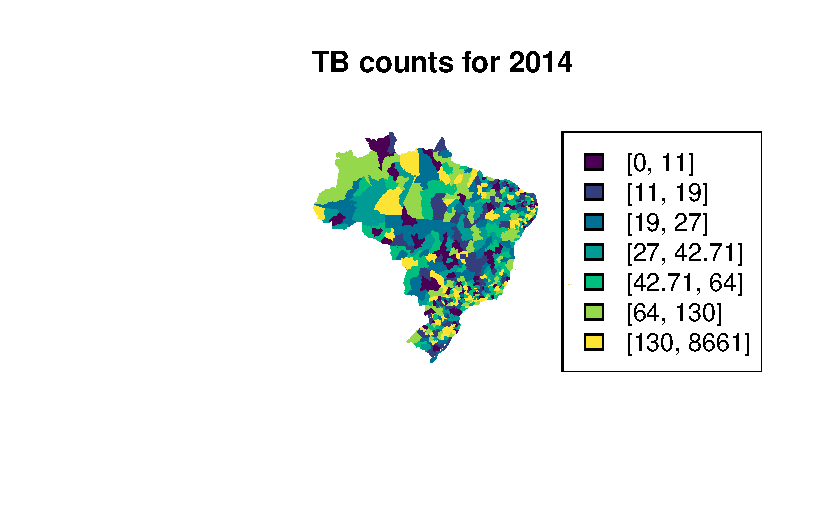
\includegraphics{Group34Coursework_files/figure-pdf/unnamed-chunk-2-1.pdf}

}

\end{figure}

\begin{Shaded}
\begin{Highlighting}[]
\FunctionTok{par}\NormalTok{(}\AttributeTok{mfrow =} \FunctionTok{c}\NormalTok{(}\DecValTok{1}\NormalTok{,}\DecValTok{1}\NormalTok{))}
\end{Highlighting}
\end{Shaded}

\hypertarget{exploratory-analyses}{%
\subsection{Exploratory analyses}\label{exploratory-analyses}}

\begin{Shaded}
\begin{Highlighting}[]
\CommentTok{\# INSERT THIS AS SUMMARY TABLE AS TABLE{-}1}
\NormalTok{summary\_table }\OtherTok{\textless{}{-}} \FunctionTok{summary}\NormalTok{(TBdata)}
\CommentTok{\# Convert the summary table to a LaTeX table using the xtable() function}
\NormalTok{latex\_table }\OtherTok{\textless{}{-}} \FunctionTok{xtable}\NormalTok{(summary\_table)}

\CommentTok{\# Print the LaTeX table to the console}
\FunctionTok{print}\NormalTok{(latex\_table)}
\end{Highlighting}
\end{Shaded}

\begin{verbatim}
% latex table generated in R 4.2.2 by xtable 1.8-4 package
% Wed Mar 22 20:19:09 2023
\begin{table}[ht]
\centering
\begin{tabular}{rllllllllllllll}
  \hline
 &   Indigenous &   Illiteracy &  Urbanisation &    Density &    Poverty & Poor\_Sanitation &  Unemployment &   Timeliness &      Year &       TB &   Population &     Region &      lon &      lat \\ 
  \hline
X & Min.   : 0.01034   & Min.   : 2.336   & Min.   :22.34   & Min.   :0.4223   & Min.   : 5.923   & Min.   : 0.0466   & Min.   : 1.128   & Min.   : 0.00   & Min.   :2012   & Min.   :   0   & Min.   :   23966   & Min.   :11001   & Min.   :-72.86   & Min.   :-32.865   \\ 
  X.1 & 1st Qu.: 0.06366   & 1st Qu.: 6.683   & 1st Qu.:58.45   & 1st Qu.:0.5166   & 1st Qu.:26.229   & 1st Qu.: 6.3903   & 1st Qu.: 5.145   & 1st Qu.:31.29   & 1st Qu.:2012   & 1st Qu.:  17   & 1st Qu.:  105054   & 1st Qu.:24007   & 1st Qu.:-50.95   & 1st Qu.:-22.278   \\ 
  X.2 & Median : 0.10577   & Median :11.516   & Median :72.66   & Median :0.5840   & Median :42.603   & Median :13.9129   & Median : 6.782   & Median :48.36   & Median :2013   & Median :  35   & Median :  180423   & Median :31028   & Median :-46.31   & Median :-15.889   \\ 
  X.3 & Mean   : 0.84307   & Mean   :14.802   & Mean   :71.96   & Mean   :0.6212   & Mean   :44.371   & Mean   :16.4490   & Mean   : 6.930   & Mean   :47.67   & Mean   :2013   & Mean   : 125   & Mean   :  357768   & Mean   :31329   & Mean   :-46.42   & Mean   :-15.240   \\ 
  X.4 & 3rd Qu.: 0.23973   & 3rd Qu.:22.844   & 3rd Qu.:86.16   & 3rd Qu.:0.6585   & 3rd Qu.:63.907   & 3rd Qu.:24.9953   & 3rd Qu.: 8.405   & 3rd Qu.:62.58   & 3rd Qu.:2014   & 3rd Qu.:  76   & 3rd Qu.:  315440   & 3rd Qu.:41007   & 3rd Qu.:-40.64   & 3rd Qu.: -7.380   \\ 
  X.5 & Max.   :50.64623   & Max.   :41.137   & Max.   :99.93   & Max.   :1.6751   & Max.   :77.883   & Max.   :58.4328   & Max.   :20.438   & Max.   :96.69   & Max.   :2014   & Max.   :9097   & Max.   :14597964   & Max.   :53001   & Max.   :-34.95   & Max.   :  3.486   \\ 
   \hline
\end{tabular}
\end{table}
\end{verbatim}

\begin{Shaded}
\begin{Highlighting}[]
\CommentTok{\# AIM TO SKIP IT AS WE HAVE ALREADY USED CORRPLOT}
\FunctionTok{plot\_histogram}\NormalTok{(TBdata)}
\end{Highlighting}
\end{Shaded}

\begin{figure}[H]

{\centering \includegraphics{Group34Coursework_files/figure-pdf/unnamed-chunk-6-1.pdf}

}

\end{figure}

//TODO talk about the histograms and relevant distributions we can
observe

Now investigating the correlation matrix of the numerical variables

\begin{Shaded}
\begin{Highlighting}[]
\CommentTok{\# NOT REQUIRED AS WE HAVE ALREADY USED CORRPLOT}
\CommentTok{\# plot\_correlation(TBdata)}
\end{Highlighting}
\end{Shaded}

As we can see from the matrix, the variable that is the most correlated
from TB is the population, with illiteracy, poor sanitation and poverty
having a negative correlation with TB.

\hypertarget{poisson-definition}{%
\subsection{Poisson definition}\label{poisson-definition}}

As the data is count data we will first fit a Poisson module since this
distribution is a good fit for the nature of the data

\begin{Shaded}
\begin{Highlighting}[]
\NormalTok{poisson\_model }\OtherTok{\textless{}{-}} \FunctionTok{gam}\NormalTok{(TB }\SpecialCharTok{\textasciitilde{}} \FunctionTok{offset}\NormalTok{(}\FunctionTok{log}\NormalTok{(Population)) }\SpecialCharTok{+} \FunctionTok{s}\NormalTok{(Indigenous, }\AttributeTok{k =} \DecValTok{20}\NormalTok{) }\SpecialCharTok{+} \FunctionTok{s}\NormalTok{(Illiteracy , }\AttributeTok{k =} \DecValTok{20}\NormalTok{) }\SpecialCharTok{+} \FunctionTok{s}\NormalTok{(Urbanisation, }\AttributeTok{k =} \DecValTok{20}\NormalTok{) }\SpecialCharTok{+} \FunctionTok{s}\NormalTok{(Density, }\AttributeTok{k =} \DecValTok{20}\NormalTok{) }\SpecialCharTok{+} \FunctionTok{s}\NormalTok{(Poverty, }\AttributeTok{k =} \DecValTok{20}\NormalTok{) }\SpecialCharTok{+} \FunctionTok{s}\NormalTok{(Poor\_Sanitation, }\AttributeTok{k =} \DecValTok{20}\NormalTok{) }\SpecialCharTok{+} \FunctionTok{s}\NormalTok{(Unemployment, }\AttributeTok{k =} \DecValTok{20}\NormalTok{) }\SpecialCharTok{+} \FunctionTok{s}\NormalTok{(Year, }\AttributeTok{k=}\DecValTok{3}\NormalTok{) }\SpecialCharTok{+} \FunctionTok{s}\NormalTok{(Timeliness, }\AttributeTok{k =} \DecValTok{20}\NormalTok{) }\SpecialCharTok{+}\FunctionTok{te}\NormalTok{(lon, Year, }\AttributeTok{k =} \DecValTok{3}\NormalTok{)}\SpecialCharTok{+} \FunctionTok{te}\NormalTok{(lat, Year, }\AttributeTok{k =} \DecValTok{3}\NormalTok{), }\AttributeTok{family =}\NormalTok{ poisson, }\AttributeTok{data =}\NormalTok{ TBdata, }\AttributeTok{method =} \StringTok{\textquotesingle{}REML\textquotesingle{}}\NormalTok{)}
\FunctionTok{summary}\NormalTok{(poisson\_model)}
\end{Highlighting}
\end{Shaded}

\begin{verbatim}

Family: poisson 
Link function: log 

Formula:
TB ~ offset(log(Population)) + s(Indigenous, k = 20) + s(Illiteracy, 
    k = 20) + s(Urbanisation, k = 20) + s(Density, k = 20) + 
    s(Poverty, k = 20) + s(Poor_Sanitation, k = 20) + s(Unemployment, 
    k = 20) + s(Year, k = 3) + s(Timeliness, k = 20) + te(lon, 
    Year, k = 3) + te(lat, Year, k = 3)

Parametric coefficients:
             Estimate Std. Error z value Pr(>|z|)    
(Intercept) -8.467263   0.004435   -1909   <2e-16 ***
---
Signif. codes:  0 '***' 0.001 '**' 0.01 '*' 0.05 '.' 0.1 ' ' 1

Approximate significance of smooth terms:
                      edf Ref.df Chi.sq p-value    
s(Indigenous)      18.393  18.92 1051.3  <2e-16 ***
s(Illiteracy)      18.157  18.89  341.5  <2e-16 ***
s(Urbanisation)    18.879  18.99 1502.8  <2e-16 ***
s(Density)         17.396  18.05 1763.1  <2e-16 ***
s(Poverty)         18.636  18.95 2027.8  <2e-16 ***
s(Poor_Sanitation) 18.327  18.91 1251.0  <2e-16 ***
s(Unemployment)    18.648  18.98 2622.8  <2e-16 ***
s(Year)             1.999   2.00 1797.0  <2e-16 ***
s(Timeliness)      18.328  18.91  927.0  <2e-16 ***
te(lon,Year)        5.980   6.00 1440.1  <2e-16 ***
te(lat,Year)        5.986   6.00 1301.2  <2e-16 ***
---
Signif. codes:  0 '***' 0.001 '**' 0.01 '*' 0.05 '.' 0.1 ' ' 1

R-sq.(adj) =  0.995   Deviance explained = 82.9%
-REML =  11564  Scale est. = 1         n = 1671
\end{verbatim}

\begin{Shaded}
\begin{Highlighting}[]
\FunctionTok{gam.check}\NormalTok{(poisson\_model)}
\end{Highlighting}
\end{Shaded}

\begin{Shaded}
\begin{Highlighting}[]
\CommentTok{\#Akaike Information Criterion:}
\NormalTok{poisson\_model}\SpecialCharTok{$}\NormalTok{aic}
\end{Highlighting}
\end{Shaded}

\begin{verbatim}
[1] 22271.66
\end{verbatim}

\begin{Shaded}
\begin{Highlighting}[]
\FunctionTok{plot}\NormalTok{(poisson\_model, }\AttributeTok{shade=}\NormalTok{T, }\AttributeTok{rug =} \ConstantTok{TRUE}\NormalTok{, }\AttributeTok{residuals =} \ConstantTok{TRUE}\NormalTok{,}
\AttributeTok{pch =} \DecValTok{1}\NormalTok{, }\AttributeTok{cex =} \FloatTok{0.5}\NormalTok{)}
\end{Highlighting}
\end{Shaded}

\begin{figure}[H]

{\centering \includegraphics{Group34Coursework_files/figure-pdf/unnamed-chunk-10-1.pdf}

}

\end{figure}

\begin{figure}[H]

{\centering \includegraphics{Group34Coursework_files/figure-pdf/unnamed-chunk-10-2.pdf}

}

\end{figure}

\begin{figure}[H]

{\centering \includegraphics{Group34Coursework_files/figure-pdf/unnamed-chunk-10-3.pdf}

}

\end{figure}

\begin{figure}[H]

{\centering \includegraphics{Group34Coursework_files/figure-pdf/unnamed-chunk-10-4.pdf}

}

\end{figure}

\begin{figure}[H]

{\centering \includegraphics{Group34Coursework_files/figure-pdf/unnamed-chunk-10-5.pdf}

}

\end{figure}

\begin{figure}[H]

{\centering \includegraphics{Group34Coursework_files/figure-pdf/unnamed-chunk-10-6.pdf}

}

\end{figure}

\begin{figure}[H]

{\centering \includegraphics{Group34Coursework_files/figure-pdf/unnamed-chunk-10-7.pdf}

}

\end{figure}

\begin{figure}[H]

{\centering \includegraphics{Group34Coursework_files/figure-pdf/unnamed-chunk-10-8.pdf}

}

\end{figure}

\begin{figure}[H]

{\centering \includegraphics{Group34Coursework_files/figure-pdf/unnamed-chunk-10-9.pdf}

}

\end{figure}

\begin{figure}[H]

{\centering \includegraphics{Group34Coursework_files/figure-pdf/unnamed-chunk-10-10.pdf}

}

\end{figure}

\begin{figure}[H]

{\centering \includegraphics{Group34Coursework_files/figure-pdf/unnamed-chunk-10-11.pdf}

}

\end{figure}

Our QQ-plot suggest that the poisson model fit deviates from the
theoretical quantiles in nearly all the values, showing a very flawed
fit. As this suggests that our current model doesn't fit the data
correctly and required an extension to our model as the Poisson GAM is
not accounted for enough deviance as seen in the residuals.

Since the model is not accounting for enough of the variance we will
check if there is a significant difference between the variance and the
mean. In this analyses we will use the Pearson estimate for the
dispersion parameter, this method allow us to estimate the amount of
extra variability, or over-dispersion in count data and therefore
analyse if the Poisson distribution assumption of equal mean and
variance holds.

\begin{Shaded}
\begin{Highlighting}[]
\CommentTok{\#Calculating Pearson estimate for dispersion parameter using Pearson residuals:}
\FunctionTok{sum}\NormalTok{(}\FunctionTok{residuals}\NormalTok{(poisson\_model, }\AttributeTok{type =} \StringTok{"pearson"}\NormalTok{)}\SpecialCharTok{\^{}}\DecValTok{2}\NormalTok{) }\SpecialCharTok{/} \FunctionTok{df.residual}\NormalTok{(poisson\_model)}
\end{Highlighting}
\end{Shaded}

\begin{verbatim}
[1] 9.353406
\end{verbatim}

\begin{Shaded}
\begin{Highlighting}[]
\CommentTok{\#The dispersion parameter should be 1, so it seems that there is substantial over{-}dispersion in the Poisson GAM.}
\end{Highlighting}
\end{Shaded}

As we can see from the dispersion parameter should be 1 for the
assumption of equal mean and variance to hold true, so it seems that
there is substantial over-dispersion in the Poisson GAM. This violates
one of the Poisson assumptions that the mean and variance are equal
therefore we will have to extend the model from e GAM Poisson to a
Negative Binomial GAM

\hypertarget{negative-binomial}{%
\subsection{Negative binomial}\label{negative-binomial}}

\begin{Shaded}
\begin{Highlighting}[]
\CommentTok{\#fitting a negative{-}binomial model to our TB data:}
\NormalTok{nb\_model }\OtherTok{\textless{}{-}} \FunctionTok{gam}\NormalTok{(TB }\SpecialCharTok{\textasciitilde{}} \FunctionTok{offset}\NormalTok{(}\FunctionTok{log}\NormalTok{(Population)) }\SpecialCharTok{+} \FunctionTok{s}\NormalTok{(Indigenous, }\AttributeTok{k =} \DecValTok{20}\NormalTok{) }\SpecialCharTok{+} \FunctionTok{s}\NormalTok{(Illiteracy , }\AttributeTok{k =} \DecValTok{20}\NormalTok{) }\SpecialCharTok{+} \FunctionTok{s}\NormalTok{(Urbanisation, }\AttributeTok{k =} \DecValTok{20}\NormalTok{) }\SpecialCharTok{+} \FunctionTok{s}\NormalTok{(Density, }\AttributeTok{k =} \DecValTok{20}\NormalTok{) }\SpecialCharTok{+} \FunctionTok{s}\NormalTok{(Poverty, }\AttributeTok{k =} \DecValTok{20}\NormalTok{) }\SpecialCharTok{+} \FunctionTok{s}\NormalTok{(Poor\_Sanitation, }\AttributeTok{k =} \DecValTok{20}\NormalTok{) }\SpecialCharTok{+} \FunctionTok{s}\NormalTok{(Unemployment, }\AttributeTok{k =} \DecValTok{20}\NormalTok{) }\SpecialCharTok{+} \FunctionTok{s}\NormalTok{(Year, }\AttributeTok{k=}\DecValTok{3}\NormalTok{) }\SpecialCharTok{+} \FunctionTok{s}\NormalTok{(Timeliness, }\AttributeTok{k =} \DecValTok{20}\NormalTok{) }\SpecialCharTok{+}\FunctionTok{te}\NormalTok{(lon, Year, }\AttributeTok{k =} \DecValTok{3}\NormalTok{)}\SpecialCharTok{+} \FunctionTok{te}\NormalTok{(lat, Year, }\AttributeTok{k =} \DecValTok{3}\NormalTok{), }\FunctionTok{negbin}\NormalTok{(}\AttributeTok{theta =} \DecValTok{9}\NormalTok{, }\AttributeTok{link =} \StringTok{"log"}\NormalTok{), }\AttributeTok{data =}\NormalTok{ TBdata, }\AttributeTok{method =} \StringTok{\textquotesingle{}REML\textquotesingle{}}\NormalTok{)}

\FunctionTok{summary}\NormalTok{(nb\_model)}
\end{Highlighting}
\end{Shaded}

\begin{verbatim}

Family: Negative Binomial(9) 
Link function: log 

Formula:
TB ~ offset(log(Population)) + s(Indigenous, k = 20) + s(Illiteracy, 
    k = 20) + s(Urbanisation, k = 20) + s(Density, k = 20) + 
    s(Poverty, k = 20) + s(Poor_Sanitation, k = 20) + s(Unemployment, 
    k = 20) + s(Year, k = 3) + s(Timeliness, k = 20) + te(lon, 
    Year, k = 3) + te(lat, Year, k = 3)

Parametric coefficients:
             Estimate Std. Error z value Pr(>|z|)    
(Intercept) -8.442775   0.009432  -895.1   <2e-16 ***
---
Signif. codes:  0 '***' 0.001 '**' 0.01 '*' 0.05 '.' 0.1 ' ' 1

Approximate significance of smooth terms:
                      edf Ref.df Chi.sq  p-value    
s(Indigenous)       1.001  1.002  22.58 1.90e-06 ***
s(Illiteracy)      10.893 13.279  37.81 0.000278 ***
s(Urbanisation)    11.070 13.410  58.68  < 2e-16 ***
s(Density)         11.231 13.495 155.64  < 2e-16 ***
s(Poverty)          7.109  8.897  36.63 2.36e-05 ***
s(Poor_Sanitation) 14.726 16.913 134.41  < 2e-16 ***
s(Unemployment)     7.203  8.927  99.22  < 2e-16 ***
s(Year)             1.986  1.998 102.59  < 2e-16 ***
s(Timeliness)       5.216  6.533  71.00  < 2e-16 ***
te(lon,Year)        5.700  5.961 101.69  < 2e-16 ***
te(lat,Year)        5.664  5.953  83.69  < 2e-16 ***
---
Signif. codes:  0 '***' 0.001 '**' 0.01 '*' 0.05 '.' 0.1 ' ' 1

R-sq.(adj) =  0.895   Deviance explained = 53.4%
-REML = 7203.2  Scale est. = 1         n = 1671
\end{verbatim}

\begin{Shaded}
\begin{Highlighting}[]
\CommentTok{\#Akaike Information Criterion}
\NormalTok{nb\_model}\SpecialCharTok{$}\NormalTok{aic}
\end{Highlighting}
\end{Shaded}

\begin{verbatim}
[1] 14199.83
\end{verbatim}

As we can see from this Akaike Information Criterion(AIC) the Negative
Binomial has a significantly lower value than the previous 18585,52 from
the GAM Poisson, meaning this is already a better fitting model than the
previous one.

Now we will check the residuals to check for any anomalies on our model
prediction

\begin{Shaded}
\begin{Highlighting}[]
\FunctionTok{gam.check}\NormalTok{(nb\_model)}
\end{Highlighting}
\end{Shaded}

\begin{figure}[H]

{\centering \includegraphics{Group34Coursework_files/figure-pdf/unnamed-chunk-14-1.pdf}

}

\end{figure}

\begin{verbatim}

Method: REML   Optimizer: outer newton
full convergence after 12 iterations.
Gradient range [-0.0002588633,5.095501e-05]
(score 7203.166 & scale 1).
Hessian positive definite, eigenvalue range [0.0002588044,2.739525].
Model rank =  167 / 167 

Basis dimension (k) checking results. Low p-value (k-index<1) may
indicate that k is too low, especially if edf is close to k'.

                      k'   edf k-index p-value    
s(Indigenous)      19.00  1.00    0.52  <2e-16 ***
s(Illiteracy)      19.00 10.89    0.51  <2e-16 ***
s(Urbanisation)    19.00 11.07    0.52  <2e-16 ***
s(Density)         19.00 11.23    0.52  <2e-16 ***
s(Poverty)         19.00  7.11    0.52  <2e-16 ***
s(Poor_Sanitation) 19.00 14.73    0.52  <2e-16 ***
s(Unemployment)    19.00  7.20    0.52  <2e-16 ***
s(Year)             2.00  1.99    0.73  <2e-16 ***
s(Timeliness)      19.00  5.22    0.57  <2e-16 ***
te(lon,Year)        6.00  5.70    0.97    0.22    
te(lat,Year)        6.00  5.66    0.96    0.12    
---
Signif. codes:  0 '***' 0.001 '**' 0.01 '*' 0.05 '.' 0.1 ' ' 1
\end{verbatim}

As we can see from the residual versus predictor plot, the values seem
to be randomly scattered with no clear trend but with some distance from
the zero line. As such we can determine that this scatter is due to
random errors and not a uncounted pattern in the model.

\begin{Shaded}
\begin{Highlighting}[]
\FunctionTok{plot}\NormalTok{(nb\_model, }\AttributeTok{shade=}\NormalTok{T, }\AttributeTok{rug =} \ConstantTok{TRUE}\NormalTok{, }\AttributeTok{residuals =} \ConstantTok{TRUE}\NormalTok{,}
\AttributeTok{pch =} \DecValTok{1}\NormalTok{, }\AttributeTok{scheme =}\DecValTok{1}\NormalTok{,  }\AttributeTok{cex =} \FloatTok{0.5}\NormalTok{)}
\end{Highlighting}
\end{Shaded}

\begin{figure}[H]

{\centering \includegraphics{Group34Coursework_files/figure-pdf/unnamed-chunk-15-1.pdf}

}

\end{figure}

\begin{figure}[H]

{\centering \includegraphics{Group34Coursework_files/figure-pdf/unnamed-chunk-15-2.pdf}

}

\end{figure}

\begin{figure}[H]

{\centering \includegraphics{Group34Coursework_files/figure-pdf/unnamed-chunk-15-3.pdf}

}

\end{figure}

\begin{figure}[H]

{\centering \includegraphics{Group34Coursework_files/figure-pdf/unnamed-chunk-15-4.pdf}

}

\end{figure}

\begin{figure}[H]

{\centering \includegraphics{Group34Coursework_files/figure-pdf/unnamed-chunk-15-5.pdf}

}

\end{figure}

\begin{figure}[H]

{\centering \includegraphics{Group34Coursework_files/figure-pdf/unnamed-chunk-15-6.pdf}

}

\end{figure}

\begin{figure}[H]

{\centering \includegraphics{Group34Coursework_files/figure-pdf/unnamed-chunk-15-7.pdf}

}

\end{figure}

\begin{figure}[H]

{\centering \includegraphics{Group34Coursework_files/figure-pdf/unnamed-chunk-15-8.pdf}

}

\end{figure}

\begin{figure}[H]

{\centering \includegraphics{Group34Coursework_files/figure-pdf/unnamed-chunk-15-9.pdf}

}

\end{figure}

\begin{figure}[H]

{\centering \includegraphics{Group34Coursework_files/figure-pdf/unnamed-chunk-15-10.pdf}

}

\end{figure}

\begin{figure}[H]

{\centering \includegraphics{Group34Coursework_files/figure-pdf/unnamed-chunk-15-11.pdf}

}

\end{figure}

The QQ-plot looks much better for the Negative Binomial model. The
majority of points lie either on top of very near the y=x line, except
for a few towards the extremes. This indicates our assumption about the
true distribution of the data is a lot more safe than it was before.

\begin{Shaded}
\begin{Highlighting}[]
\CommentTok{\#Calculating Pearson estimate for dispersion parameter using Pearson residuals:}
\FunctionTok{sum}\NormalTok{(}\FunctionTok{residuals}\NormalTok{(nb\_model, }\AttributeTok{type =} \StringTok{"pearson"}\NormalTok{)}\SpecialCharTok{\^{}}\DecValTok{2}\NormalTok{) }\SpecialCharTok{/} \FunctionTok{df.residual}\NormalTok{(nb\_model)}
\end{Highlighting}
\end{Shaded}

\begin{verbatim}
[1] 1.338156
\end{verbatim}

The dispersion parameter is very close to 1, unlike for the Poisson
model, meaning that the model that can account for most of the
over-dispersion in the data. As such a dispersion parameter value close
to 1 can be interpreted as the model is a good fit for the data due to
the model adequately capture the variability of the the response
variable.

\hypertarget{again-tidy-up-the-plots-of-the-negative-binomial}{%
\subsection{Again tidy up the plots of the Negative
Binomial}\label{again-tidy-up-the-plots-of-the-negative-binomial}}

\begin{Shaded}
\begin{Highlighting}[]
\FunctionTok{plot}\NormalTok{(nb\_model, }\AttributeTok{shade=}\NormalTok{T, }\AttributeTok{rug =} \ConstantTok{TRUE}\NormalTok{, }\AttributeTok{residuals =} \ConstantTok{TRUE}\NormalTok{,}\AttributeTok{scheme=}\DecValTok{1}\NormalTok{,}
\AttributeTok{pch =} \DecValTok{1}\NormalTok{, }\AttributeTok{cex =} \FloatTok{0.5}\NormalTok{)}
\end{Highlighting}
\end{Shaded}

\begin{figure}[H]

{\centering \includegraphics{Group34Coursework_files/figure-pdf/unnamed-chunk-17-1.pdf}

}

\end{figure}

\begin{figure}[H]

{\centering \includegraphics{Group34Coursework_files/figure-pdf/unnamed-chunk-17-2.pdf}

}

\end{figure}

\begin{figure}[H]

{\centering \includegraphics{Group34Coursework_files/figure-pdf/unnamed-chunk-17-3.pdf}

}

\end{figure}

\begin{figure}[H]

{\centering \includegraphics{Group34Coursework_files/figure-pdf/unnamed-chunk-17-4.pdf}

}

\end{figure}

\begin{figure}[H]

{\centering \includegraphics{Group34Coursework_files/figure-pdf/unnamed-chunk-17-5.pdf}

}

\end{figure}

\begin{figure}[H]

{\centering \includegraphics{Group34Coursework_files/figure-pdf/unnamed-chunk-17-6.pdf}

}

\end{figure}

\begin{figure}[H]

{\centering \includegraphics{Group34Coursework_files/figure-pdf/unnamed-chunk-17-7.pdf}

}

\end{figure}

\begin{figure}[H]

{\centering \includegraphics{Group34Coursework_files/figure-pdf/unnamed-chunk-17-8.pdf}

}

\end{figure}

\begin{figure}[H]

{\centering \includegraphics{Group34Coursework_files/figure-pdf/unnamed-chunk-17-9.pdf}

}

\end{figure}

\begin{figure}[H]

{\centering \includegraphics{Group34Coursework_files/figure-pdf/unnamed-chunk-17-10.pdf}

}

\end{figure}

\begin{figure}[H]

{\centering \includegraphics{Group34Coursework_files/figure-pdf/unnamed-chunk-17-11.pdf}

}

\end{figure}

\begin{Shaded}
\begin{Highlighting}[]
\FunctionTok{plot}\NormalTok{(nb\_model, }\AttributeTok{shade =}\NormalTok{ T, }\AttributeTok{rug =} \ConstantTok{TRUE}\NormalTok{, }\AttributeTok{residuals =} \ConstantTok{TRUE}\NormalTok{, }\AttributeTok{scheme =} \DecValTok{2}\NormalTok{, }\AttributeTok{pch =} \DecValTok{1}\NormalTok{,}
    \AttributeTok{cex =} \FloatTok{0.5}\NormalTok{)}
\end{Highlighting}
\end{Shaded}

\begin{figure}[H]

{\centering \includegraphics{Group34Coursework_files/figure-pdf/unnamed-chunk-18-1.pdf}

}

\end{figure}

\begin{figure}[H]

{\centering \includegraphics{Group34Coursework_files/figure-pdf/unnamed-chunk-18-2.pdf}

}

\end{figure}

\begin{figure}[H]

{\centering \includegraphics{Group34Coursework_files/figure-pdf/unnamed-chunk-18-3.pdf}

}

\end{figure}

\begin{figure}[H]

{\centering \includegraphics{Group34Coursework_files/figure-pdf/unnamed-chunk-18-4.pdf}

}

\end{figure}

\begin{figure}[H]

{\centering \includegraphics{Group34Coursework_files/figure-pdf/unnamed-chunk-18-5.pdf}

}

\end{figure}

\begin{figure}[H]

{\centering \includegraphics{Group34Coursework_files/figure-pdf/unnamed-chunk-18-6.pdf}

}

\end{figure}

\begin{figure}[H]

{\centering \includegraphics{Group34Coursework_files/figure-pdf/unnamed-chunk-18-7.pdf}

}

\end{figure}

\begin{figure}[H]

{\centering \includegraphics{Group34Coursework_files/figure-pdf/unnamed-chunk-18-8.pdf}

}

\end{figure}

\begin{figure}[H]

{\centering \includegraphics{Group34Coursework_files/figure-pdf/unnamed-chunk-18-9.pdf}

}

\end{figure}

\begin{figure}[H]

{\centering \includegraphics{Group34Coursework_files/figure-pdf/unnamed-chunk-18-10.pdf}

}

\end{figure}

\begin{figure}[H]

{\centering \includegraphics{Group34Coursework_files/figure-pdf/unnamed-chunk-18-11.pdf}

}

\end{figure}

\begin{Shaded}
\begin{Highlighting}[]
\FunctionTok{par}\NormalTok{(}\AttributeTok{mfrow =} \FunctionTok{c}\NormalTok{(}\DecValTok{1}\NormalTok{, }\DecValTok{2}\NormalTok{))}

\FunctionTok{qq.gam}\NormalTok{(poisson\_model, }\AttributeTok{main =} \StringTok{"Q{-}Q Plot for Poisson Model"}\NormalTok{)}
\FunctionTok{qq.gam}\NormalTok{(nb\_model, }\AttributeTok{main =} \StringTok{"Q{-}Q Plot for Negative Binomial Model"}\NormalTok{)}
\end{Highlighting}
\end{Shaded}

\begin{figure}[H]

{\centering \includegraphics{Group34Coursework_files/figure-pdf/unnamed-chunk-19-1.pdf}

}

\end{figure}

\begin{Shaded}
\begin{Highlighting}[]
\NormalTok{preds }\OtherTok{=} \FunctionTok{predict}\NormalTok{(nb\_model, }\AttributeTok{type =} \StringTok{"terms"}\NormalTok{, }\AttributeTok{se.fit =} \ConstantTok{FALSE}\NormalTok{)}
\NormalTok{year2012 }\OtherTok{\textless{}{-}}\NormalTok{ preds[}\DecValTok{1}\SpecialCharTok{:}\DecValTok{557}\NormalTok{, ]}
\NormalTok{year2013 }\OtherTok{\textless{}{-}}\NormalTok{ preds[}\DecValTok{558}\SpecialCharTok{:}\DecValTok{1114}\NormalTok{, ]}
\NormalTok{year2014 }\OtherTok{\textless{}{-}}\NormalTok{ preds[}\DecValTok{1115}\SpecialCharTok{:}\DecValTok{1671}\NormalTok{, ]}
\NormalTok{cord.pred\_2012 }\OtherTok{\textless{}{-}} \FunctionTok{as.numeric}\NormalTok{(year2012[, }\DecValTok{8}\NormalTok{])}
\NormalTok{cord.pred\_2013 }\OtherTok{\textless{}{-}} \FunctionTok{as.numeric}\NormalTok{(year2013[, }\DecValTok{9}\NormalTok{])}
\NormalTok{cord.pred\_2014 }\OtherTok{\textless{}{-}} \FunctionTok{as.numeric}\NormalTok{(year2014[, }\DecValTok{10}\NormalTok{])}
\NormalTok{List }\OtherTok{=} \FunctionTok{list}\NormalTok{(cord.pred\_2012, cord.pred\_2013, cord.pred\_2014)}
\NormalTok{cord.preds.mean }\OtherTok{\textless{}{-}} \FunctionTok{rowMeans}\NormalTok{(}\FunctionTok{simplify2array}\NormalTok{(List))}
\NormalTok{cord.change\_1 }\OtherTok{\textless{}{-}}\NormalTok{ cord.pred\_2013 }\SpecialCharTok{{-}}\NormalTok{ cord.pred\_2012}
\NormalTok{cord.change\_2 }\OtherTok{\textless{}{-}}\NormalTok{ cord.pred\_2014 }\SpecialCharTok{{-}}\NormalTok{ cord.pred\_2013}
\end{Highlighting}
\end{Shaded}

\begin{Shaded}
\begin{Highlighting}[]
\FunctionTok{plot.map}\NormalTok{(cord.pred\_2012, }\AttributeTok{n.levels =} \DecValTok{8}\NormalTok{, }\AttributeTok{main =} \StringTok{"Predicted TB risk in 2012"}\NormalTok{)}
\end{Highlighting}
\end{Shaded}

\begin{figure}[H]

{\centering \includegraphics{Group34Coursework_files/figure-pdf/unnamed-chunk-21-1.pdf}

}

\end{figure}

\begin{Shaded}
\begin{Highlighting}[]
\FunctionTok{plot.map}\NormalTok{(cord.pred\_2013, }\AttributeTok{n.levels =} \DecValTok{8}\NormalTok{, }\AttributeTok{main =} \StringTok{"Predicted TB risk in 2013"}\NormalTok{)}
\end{Highlighting}
\end{Shaded}

\begin{figure}[H]

{\centering \includegraphics{Group34Coursework_files/figure-pdf/unnamed-chunk-22-1.pdf}

}

\end{figure}

\hypertarget{refs}{}
\begin{CSLReferences}{1}{0}
\leavevmode\vadjust pre{\hypertarget{ref-who_tb_2020}{}}%
\emph{Global Tuberculosis Report 2020}. 2020. Gen{è}ve, Switzerland:
World Health Organization.

\end{CSLReferences}



\end{document}
